\documentclass[tikz]{standalone}

\usepackage[latin1]{inputenc}
\usepackage{tikz}

% GNUPL
\begin{document}
\pagestyle{empty}


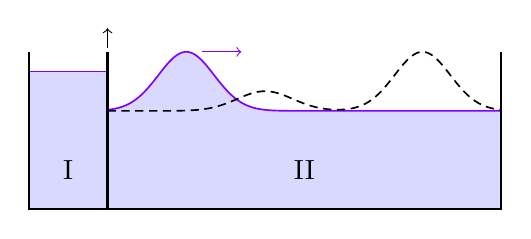
\begin{tikzpicture}
    %\draw[very thin,color=gray] (-1,1.1) grid (3.9,3.9);
    % \draw[->] (-1.1,0) -- (3,0) node[right] {$x$};
    % \draw[->] (0,-0.2) -- (0,2) node[above] {$U$};
    % \draw[->] (4,3) -- (5,3);
    \draw [draw=none, fill=blue!15, domain=0:5,samples=200] plot (\x,  {0.75*exp(-((\x-1)*2)^2)+0.25}) -- (5,-1) -- (0,-1) -- cycle;

    \draw[->,blue!50!magenta] (1.2,1) -- ++(0.5,0);

    \draw [blue!50!magenta, semithick, domain=0:5,samples=200] plot (\x,  {0.75*exp(-((\x-1)*2)^2)+0.25});

    \draw [draw=none, fill=blue!15]  (0,-1) rectangle (-1,0.75);
    \draw [blue!50!magenta,semithick] (-1,0.75) -- (0,0.75);
    \draw[thick,black] (0,1) -- (0,-1) -- (5,-1) -- (5,1); 
    \draw[thick,black] (0,-1) -- (-1,-1) -- (-1,1);

    \draw[->] (0,1.05) -- ++(0,0.25);

    \draw (-0.5,-0.5) node {I};
    \draw (2.5,-0.5) node {II};

  \draw [black, densely dashed, semithick, domain=0:5,samples=200] plot (\x,  {0.25*exp(-((\x-2)*2)^2)+0.25+0.75*exp(-((\x-4)*2)^2)});
% \draw [black, semithick, domain=-1:15,samples=200] plot (\x,  {2*exp(-(\x-3)^2/5)+4*exp(-(\x-8)^2/3)+6*exp(-(\x-12)^2)});

\end{tikzpicture}


\end{document}